\chapter{Database Design}

\section{Entities, Attributes and Relationships}
The database, called data, will have seven tables, teacher, student, class, subjects, courses, marksheet and branch. Each will hold information about either the student or teacher. The two
tables will be linked through a foreign key. The student table has the following fields:\\
\begin{figure}[H]
\centering
\caption{student table}
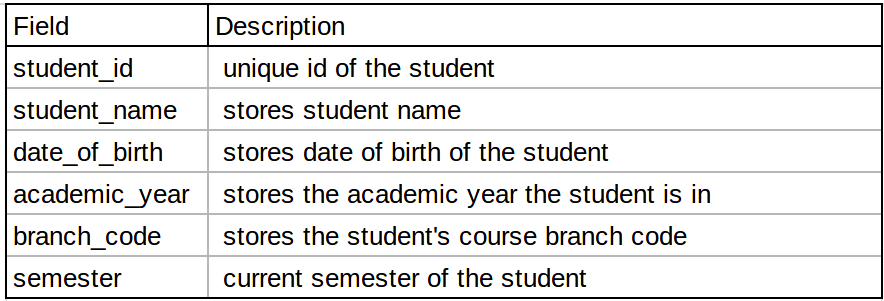
\includegraphics[scale=.5]{./StudentTable.png}
\\[0.2in]
\label{fig:Student Table}
\end{figure}
Since one teacher can teach many students, We thought it only right to insert a foreign key
branch\_code and semester into the student table. In addition, we have made the teacher account to have admin privilege. This will
enable us to focus more on the programming than on particulars of the database.\\
\pagebreak
\thispagestyle{fancy}
\section{Identify Major entities, attributes and relationships}
\begin{itemize}
\item Login page to give access to priviledged teachers.
\item Adding student and teacher details by the teacher.
\item Changing the id and password of the teacher.
which stores the details of transaction.
\item Teachers can check all details butnot passwords and modify them.
\item Teacher can delete the entities in the tables.
\item Easy  search facilities to get the reqiured information.
\end{itemize}

\thispagestyle{fancy}

\section{ER Schema}
\begin{figure}[H]
\centering
\caption{Entity Relationship Diagram}
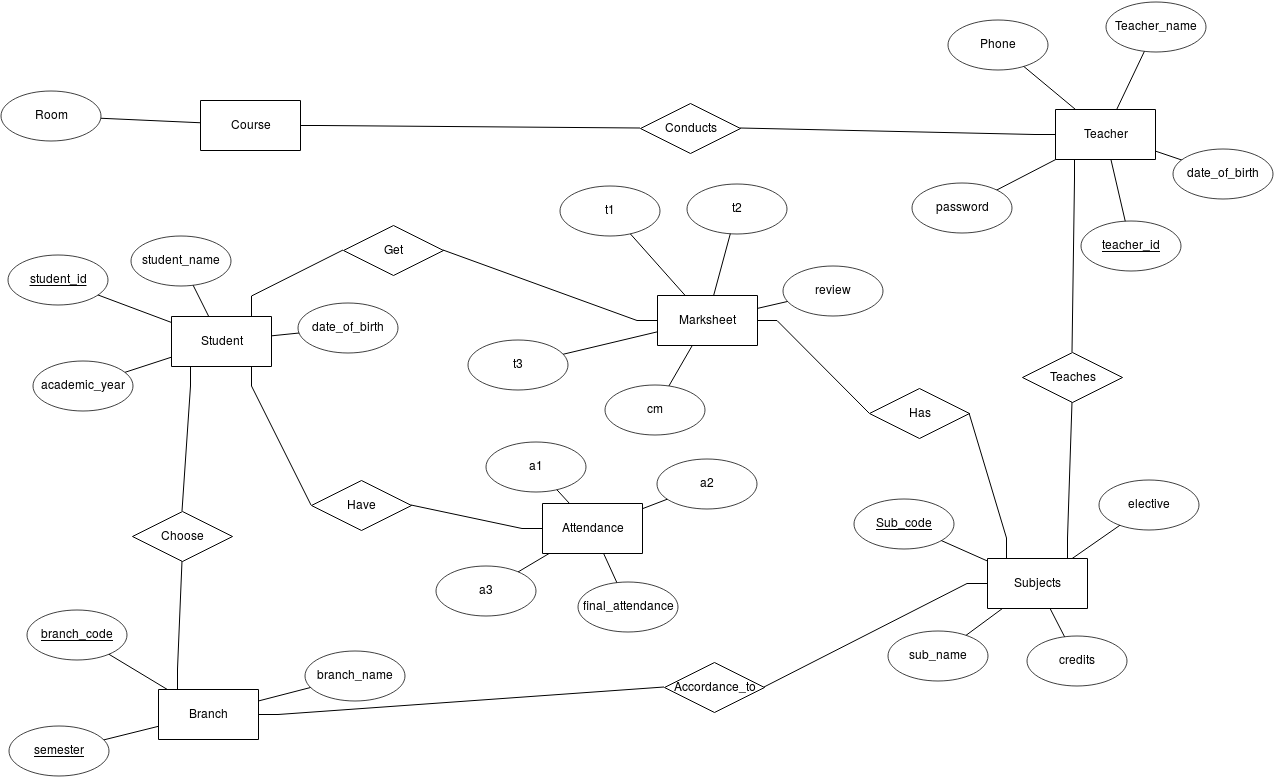
\includegraphics[scale=.35]{./erd.png}
\\[0.2in]
\label{fig:Entitiy Relationship Diagram}
\end{figure}

\pagebreak
\thispagestyle{fancy}

\section{Schema Diagram}
\begin{figure}[H]
\centering
\caption{Relational Schema}
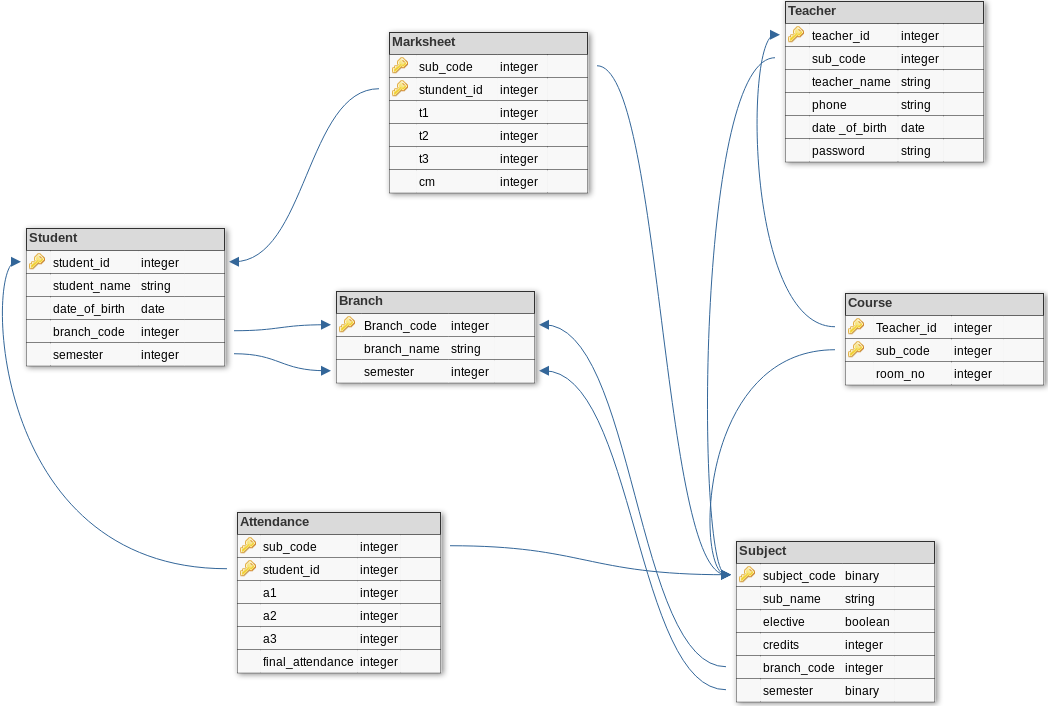
\includegraphics[scale=.5]{./schema.png}
\\[0.2in]
\label{fig:Relational Schema}
\end{figure}

\thispagestyle{fancy}